% Define the layers to draw the diagram
\pgfdeclarelayer{background}
\pgfdeclarelayer{background1}
\pgfdeclarelayer{foreground}
\pgfsetlayers{background,background1,main,foreground}

% Define block styles
\tikzstyle{nodeStyle} = [draw, text width=6cm,  minimum height=1.75em, text centered]
\tikzstyle{port} = [draw, fill={rgb,255:red,135; green,220; blue,170}, text width=0.75cm, font=\fontsize{6}{7.2}\sffamily, text centered]
\tikzstyle{FU} = [draw, fill={rgb,255:red,212; green,170; blue,0}, text width=5.0em, font=\fontsize{6}{7.2}\sffamily, rotate=90, text centered]
\tikzstyle{arrow} = [draw, thick, color=black!80, font=\footnotesize\sffamily]
\usetikzlibrary{calc}

% Draw background
\newcommand{\background}[7]{%
    \begin{pgfonlayer}{background}
        % Left-top corner of the background rectangle
        \path (#1.west |- #2.north)+(-1,0.4) node (a1) {};
        % Right-bottom corner of the background rectangle
        \path (#3.east |- #4.south)+(+0.4,#5) node (a2) {};
        % Draw the background
        \path[fill=#6, draw=black!50]
        (a1) rectangle (a2);
        \path let \p{x}=(a1), \p{y}=($(a1)!0.5!(a2)$) in (\x{x}, \y{y})+(0.5,0) node (u1)[rotate=90]
        {#7};
\end{pgfonlayer}}

\begin{wrapfigure}[25]{l}{0.6\textwidth}
    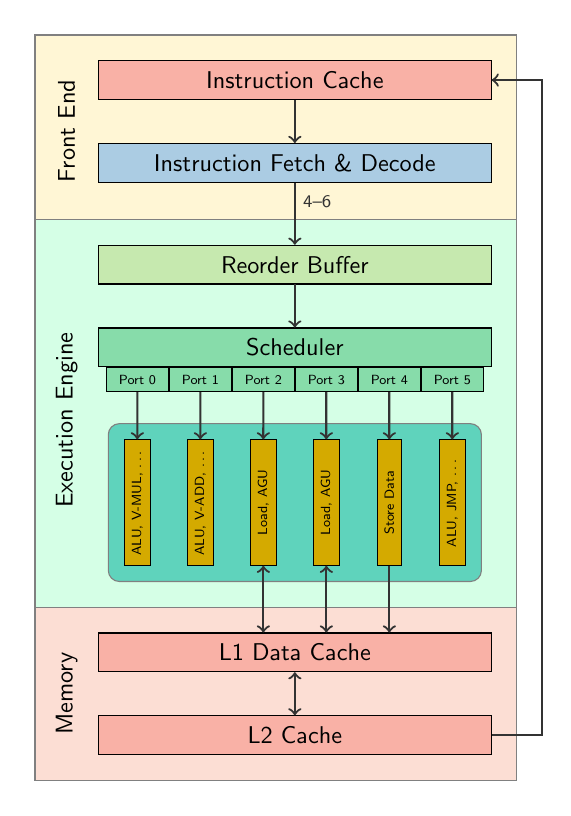
\begin{tikzpicture}[scale=0.8,transform shape,font=\fontsize{11}{13.2}\sffamily]
    % Draw diagram elements
    \path node (nIC) [nodeStyle, fill={rgb,255:red,249; green,177; blue,166}] {Instruction Cache};
    \path (nIC.south)+(0.0,-1.0) node (nFD) [nodeStyle, fill={rgb,255:red,171; green,204; blue,227}] {Instruction Fetch \& Decode};
    \path (nFD.south)+(0.0,-1.3) node (nReorder) [nodeStyle, fill={rgb,255:red,198; green,233; blue,175}] {Reorder Buffer};
    \path (nReorder.south)+(0.0,-1.0) node (nRS) [nodeStyle, fill={rgb,255:red,135; green,220; blue,170}] {Scheduler};
    \path (nRS.south)+(-2.5,0.0) node[anchor=north] (nPort0) [port] {Port 0};
    \path (nRS.south)+(-1.5,0.0) node[anchor=north] (nPort1) [port] {Port 1};
    \path (nRS.south)+(-0.5,0.0) node[anchor=north] (nPort2) [port] {Port 2};
    \path (nRS.south)+(0.5,0.0) node[anchor=north] (nPort3) [port] {Port 3};
    \path (nRS.south)+(1.5,0.0) node[anchor=north] (nPort4) [port] {Port 4};
    \path (nRS.south)+(2.5,0.0) node[anchor=north] (nPort5) [port] {Port 5};
    
    \path (nPort0.south)+(0,-0.75) node[anchor=east] (nPort0FU) [FU] {ALU, V-MUL, \dots};
    \path (nPort1.south)+(0,-0.75) node[anchor=east] (nPort1FU) [FU] {ALU, V-ADD, \dots};
    \path (nPort2.south)+(0,-0.75) node[anchor=east] (nPort2FU) [FU] {Load, AGU};
    \path (nPort3.south)+(0,-0.75) node[anchor=east] (nPort3FU) [FU] {Load, AGU};
    \path (nPort4.south)+(0,-0.75) node[anchor=east] (nPort4FU) [FU] {Store Data};
    \path (nPort5.south)+(0,-0.75) node[anchor=east] (nPort5FU) [FU] {ALU, JMP, \dots};
    
    \begin{pgfonlayer}{background1}
    \path (nPort0FU.north |- nPort0FU.east)+(-0.25,0.25) node (ee_tl) {};
    \path (nPort5FU.south |- nPort5FU.west)+(+0.25,-0.25) node (ee_br) {};
    \path[fill={rgb,255:red,95; green,211; blue,188}, draw=black!50, rounded corners] (ee_tl) rectangle (ee_br);
    \end{pgfonlayer}
    
    \path let \p{x}=(nRS.south), \p{y}=(ee_br.south) in (\x{x}, \y{y})+(0,-1.0) node (nL1D)
    [nodeStyle, fill={rgb,255:red,249; green,177; blue,166}] {L1 Data Cache};
    \path (nL1D.south)+(0.0,-1.0) node (nL2) [nodeStyle, fill={rgb,255:red,249; green,177; blue,166}] {L2 Cache};
    
    % Draw arrows between elements
    \draw [->, arrow] (nIC.south) -- (nFD.north);
    \draw [->, arrow] (nFD.south) -- node [right] {4--6 \textnormal\microops} +(0,-0.6) -- (nReorder.north);
    \draw [->, arrow] (nReorder.south) -- node [right] {\textnormal\microops} (nRS.north);
    
    \draw [->, arrow, font=\fontsize{6}{7.2}\sffamily] (nPort0.south) -- node [right] {\textnormal\microop} +(-0,-0.5) -- (nPort0FU.east);
    \draw [->, arrow, font=\fontsize{6}{7.2}\sffamily] (nPort1.south) -- node [right] {\textnormal\microop} +(-0,-0.5) -- (nPort1FU.east);
    \draw [->, arrow, font=\fontsize{6}{7.2}\sffamily] (nPort2.south) -- node [right] {\textnormal\microop} +(-0,-0.5) -- (nPort2FU.east);
    \draw [->, arrow, font=\fontsize{6}{7.2}\sffamily] (nPort3.south) -- node [right] {\textnormal\microop} +(-0,-0.5) -- (nPort3FU.east);
    \draw [->, arrow, font=\fontsize{6}{7.2}\sffamily] (nPort4.south) -- node [right] {\textnormal\microop} +(-0,-0.5) -- (nPort4FU.east);
    \draw [->, arrow, font=\fontsize{6}{7.2}\sffamily] (nPort5.south) -- node [right] {\textnormal\microop} +(-0,-0.5) -- (nPort5FU.east);
    
    \draw [<->, arrow] (nPort2FU.west) -- (nPort2FU.west |- nL1D.north);
    \draw [<->, arrow] (nPort3FU.west) -- (nPort3FU.west |- nL1D.north);
    \draw [->, arrow] (nPort4FU.west) -- (nPort4FU.west |- nL1D.north);
    
    \draw [<->, arrow] (nL1D.south) -- (nL2.north);
    \draw [->, arrow] (nL2.east) -- +(+0.8,-0.0) |- (nIC.east);
    
    \background{nIC}{nIC}{nL2}{nFD}{-0.7}{{rgb,255:red,255; green,246; blue,213}}{Front End}
    \background{nReorder}{nReorder}{nL2}{ee_br}{-0.5}{{rgb,255:red,213; green,255; blue,230}}{Execution Engine}
    \background{nL1D}{nL1D}{nL1D}{nL2}{-0.4}{{rgb,255:red,252; green,222; blue,212}}{Memory}
    \end{tikzpicture}
    %\caption[caption]{This is the caption\\\hspace{\textwidth}This is the second line}
    \caption[caption]{Pipeline of Intel Core\\\phantom{Figure 1.1: }CPUs (simplified). \cite{Andreas}}
    \label{fig:Pipeline}
\end{wrapfigure} 
